\let\negmedspace\undefined
\let\negthickspace\undefined
\documentclass[journal]{IEEEtran}
\usepackage[a5paper, margin=10mm, onecolumn]{geometry}
%\usepackage{lmodern} % Ensure lmodern is loaded for pdflatex
\usepackage{tfrupee} % Include tfrupee package

\setlength{\headheight}{1cm} % Set the height of the header box
\setlength{\headsep}{0mm}     % Set the distance between the header box and the top of the text

\usepackage{gvv-book}
\usepackage{gvv}
\usepackage{cite}
\usepackage{amsmath,amssymb,amsfonts,amsthm}
\usepackage{algorithmic}
\usepackage{graphicx}
\usepackage{textcomp}
\usepackage{xcolor}
\usepackage{txfonts}
\usepackage{listings}
\usepackage{enumitem}
\usepackage{mathtools}
\usepackage{gensymb}
\usepackage{comment}
\usepackage[breaklinks=true]{hyperref}
\usepackage{tkz-euclide} 
\usepackage{listings}
% \usepackage{gvv}                                        
\def\inputGnumericTable{}                                 
\usepackage[latin1]{inputenc}                                
\usepackage{color}                                            
\usepackage{array}                                            
\usepackage{longtable}                                       
\usepackage{calc}                                             
\usepackage{multirow}                                         
\usepackage{hhline}                                           
\usepackage{ifthen}                                           
\usepackage{lscape}
\usepackage{circuitikz}
\tikzstyle{block} = [rectangle, draw, fill=blue!20, 
    text width=4em, text centered, rounded corners, minimum height=3em]
\tikzstyle{sum} = [draw, fill=blue!10, circle, minimum size=1cm, node distance=1.5cm]
\tikzstyle{input} = [coordinate]
\tikzstyle{output} = [coordinate]


\begin{document}

\bibliographystyle{IEEEtran}
\vspace{3cm}

\title{2.10.19}
\author{AI25BTECH110031 \\ Shivam Sawarkar}
 \maketitle
% \newpage
% \bigskip
{\let\newpage\relax\maketitle}

\renewcommand{\thefigure}{\theenumi}
\renewcommand{\thetable}{\theenumi}
\setlength{\intextsep}{10pt} % Space between text and floats


\numberwithin{equation}{section}
\numberwithin{figure}{enumi}
\renewcommand{\thetable}{\theenumi}

\textbf{Question(2.10.19)}
 For three vectors $\Vec{u},\Vec{v},\vec{w}$ which of the following expression is not equal to any of the
 remaining three?
 \begin{enumerate}[label=\alph*]
     \item $\vec{u}\cdot(\vec{v}\times\vec{w})$
     \item $\vec{v}\cdot(\vec{u}\times\vec{w})$
     \item $(\vec{v}\times\vec{w})\cdot\vec{u}$
     \item $(\vec{u}\times\vec{v})\cdot\vec{w}$
 \end{enumerate}

 \textbf{Solution}
 As we know that dot product is cumulative $(1)$ and $(2)$ are equal \\
 That is,
\begin{align}
     \vec{u}^\top(\vec{v}\times\vec{w}) = (\vec{v}\times\vec{w})^\top\vec{u}
\end{align}

We prove
\begin{align}
\vec{u}^\top(\vec{v}\times\vec{w})=(\vec{u}\times\vec{v})^\top\vec{w}
\end{align}
using the cross-product (skew-)matrix.

Define, for \(\vec{a}=(a_1,a_2,a_3)^T\),
\begin{align}
S(\vec{a})=\myvec{
0 & -a_3 & a_2\\
a_3 & 0 & -a_1\\
-a_2 & a_1 & 0
}
\end{align}

which satisfies $(\vec{a})\vec{b}=\vec{a}\times\vec{b}$  for all $\vec{b}\in\mathbb{R}^3$.


\begin{align}
\vec{u}^\top(\vec{v}\times\vec{w})
&= \vec{u}^T\big(S(\vec{v})\vec{w}\big)
\quad\text{(since }S(\vec{v})\vec{w}=\vec{v}\times\vec{w}\text{)}\\ 
&= \big(\vec{u}^T S(\vec{v})\big)\vec{w} \\ 
&= \big(S(\vec{v})^T\vec{u}\big)^T\vec{w}
\quad\text{(transpose identity: }(A^T x)^T = x^T A\text{)}\\ 
&= \big(-S(\vec{v})\vec{u}\big)^T\vec{w}
\quad\text{(since }S(\vec{v})^T=-S(\vec{v})\text{)}\\ 
&= \big(\vec{u}\times\vec{v}\big)^T\vec{w}
\quad\text{(because }-S(\vec{v})\vec{u} = -(\vec{v}\times\vec{u}) = \vec{u}\times\vec{v})
\end{align}

Thus
\begin{align}
\vec{u}^\top(\vec{v}\times\vec{w}) = (\vec{u}\times\vec{v})^\top\vec{w}
\end{align}

This shows that (a), (c) and (d) are equal \\ 

For example,
Let
\begin{align}
\vec{u}=\myvec{1 \\ -1 \\ 1}, \quad \vec{v}=\myvec{0 \\ 1 \\ 2}, \quad \vec{w}=\myvec{1 \\ 0 \\ -1}.
\end{align}

Case 1: $\vec{u} ^\top (\vec{v} \times \vec{w})$

\begin{align}
\vec{v} \times \vec{w} =
\myvec{
v_{23} & w_{23} \\
v_{31} & w_{31} \\
v_{12} & w_{12}
}
=
\myvec{
v_2 w_3 - v_3 w_2 \\
v_3 w_1 - v_1 w_3 \\
v_1 w_2 - v_2 w_1
}
=
\myvec{
1 \times (-1) - 2 \times 0 \\
2 \times 1 - 0 \times (-1) \\
0 \times 0 - 1 \times 1
}
\end{align}


So
\begin{align}
\vec{v}\times \vec{w} = \myvec{-1 \\ 2 \\ -1}
\end{align}

Now compute the dot product:
\begin{align}
\vec{u} ^\top (\vec{v}\times \vec{w}) &= \myvec{1 & -1 & 1}\myvec{-1 \\ 2 \\ -1} \\
&= (1)(-1) + (-1)(2) + (1)(-1) \\
&= -4
\end{align}

\begin{align}
\boxed{\vec{u}^\top(\vec{v}\times \vec{w}) = -4}
\end{align}

Case 2: $\vec{v} ^\top (\vec{u} \times \vec{w})$

Compute $\vec{u} \times \vec{w}$:
\begin{align}
\vec{u} \times \vec{w} =
\myvec{
u_{23} & w_{23} \\
u_{31} & w_{31} \\
u_{12} & w_{12}
}
=
\myvec{
u_2 w_3 - u_3 w_2 \\
u_3 w_1 - u_1 w_3 \\
u_1 w_2 - u_2 w_1
}
=
\myvec{
(-1) \times (-1) - 1 \times 0 \\
1 \times 1 - 1 \times (-1) \\
1 \times 0 - (-1) \times 1
}
\end{align}

So
\begin{align}
\vec{u}\times \vec{w} = \myvec{1 \\ 2 \\ 1}.
\end{align}

Now compute dot product:
\begin{align}
\vec{v}^\top(\vec{u}\times \vec{w}) &= \myvec{0 & 1 & 2}\myvec{1 \\ 2 \\ 1} \\
&= (0)(1) + (1)(2) + (2)(1) \\
&= 4.
\end{align}

\begin{align}
\boxed{\vec{u}^\top(\vec{u}\times \vec{w}) = 4}
\end{align}

Case 3: $(\vec{v} \times \vec{w}) ^\top \vec{u}$

We already have
\begin{align}
\vec{v}\times \vec{w} = \myvec{-1 \\ 2 \\ -1}
\end{align}

Now compute:
\begin{align}
(\vec{v}\times \vec{w})^\top \vec{u} &= \myvec{-1 & 2 & -1}\myvec{1 \\ -1 \\ 1} \\
&= (-1)(1) + (2)(-1) + (-1)(1) \\
&= -4.
\end{align}

\begin{align}
\boxed{(\vec{v}\times \vec{w})^\top \vec{u} = -4}
\end{align}

Case 4: $(\vec{u} \times \vec{v})^\top \vec{w}$

Compute $\vec{u} \times \vec{v}$:
\begin{align}
\vec{u} \times \vec{v} =
\myvec{
u_{23} & v_{23} \\
u_{31} & v_{31} \\
u_{12} & v_{12}
}
=
\myvec{
u_2 v_3 - u_3 v_2 \\
u_3 v_1 - u_1 v_3 \\
u_1 v_2 - u_2 v_1
}
=
\myvec{
(-1) \times 2 - 1 \times 1 \\
1 \times 0 - (-1) \times 2 \\
1 \times 1 - (-1) \times 0
}
\end{align}

So
\begin{align}
\vec{u}\times \vec{v} =\myvec{-3 \\ -2 \\ 1}
\end{align}

Now compute:
\begin{align}
(\vec{u}\times \vec{v})^\top \vec{w} &= \myvec{-3 & -2 & 1}\myvec{1 \\ 0 \\ -1} \\
&= (-3)(1) + (-2)(0) + (1)(-1) \\
&= -3 + 0 - 1 = -4.
\end{align}

\begin{align}
\boxed{(\vec{u}\times \vec{v})^\top \vec{w} = -4}
\end{align}

Final Results
\begin{align}
\vec{u}^\top(\vec{v}\times \vec{w})=-4,\quad
\vec{v}^\top(\vec{u}\times \vec{w})=4,\quad
(\vec{v}\times \vec{w})^\top \vec{u}=-4,\quad
(\vec{u}\times \vec{v})^\top \vec{w}=-4
\end{align}

Thus (a), (c) and (d) are same

\begin{figure}
    \centering
    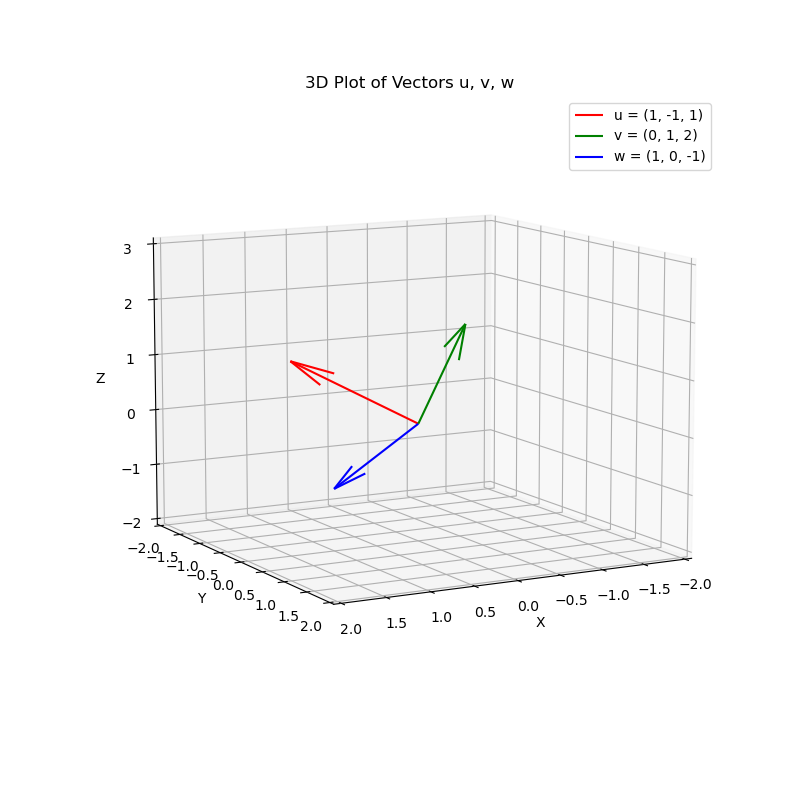
\includegraphics[width=1\linewidth]{figs/plot5.png}
    \caption{}
    \label{fig:placeholder}
\end{figure}






\end{document}